\documentclass[a4paper,12pt]{book}
\usepackage[utf8]{inputenc}
\usepackage{graphicx}
\usepackage{tikz}
\usetikzlibrary{arrows,shapes.geometric,shapes.gates.logic,automata}
\usepackage[style=verbose-ibid,backend=biber]{biblatex}
\usepackage{hyperref}

% Code style
\usepackage{listings}
\usepackage{color}
\definecolor{lightgray}{gray}{0.9}

\lstset{
    showstringspaces=false,
    basicstyle=\ttfamily,
    keywordstyle=\color{blue},
    commentstyle=\color[grey]{0.6},
    stringstyle=\color[RGB]{255,150,75}
}

\newcommand{\inlinecode}[2][Verilog]{\colorbox{lightgray}{\lstinline[language=#1]$#2$}}
% /Code style

%\setcounter{secnumdepth}{3}
%\setcounter{tocdepth}{3}
\usepackage{prettyref}
\usepackage{units}
\usepackage{amsmath}

\addbibresource{./references.bib}
\begin{document}

\author{John R. Moser}
\title{The Kerberos RISC-V Core}
\date{May 2020}

\frontmatter
\maketitle
\chapter*{Preface}
This book documents the design of the Taiga and Kerberos RISC-V cores.  Kerberos implements RV32I and RV64I, plus the multiply and divide extension, atomics, single- and double-precision floating point operations, 16-bit compressed instructions, Zicsr, and Zifenci.  Together, this is called RV64IMAFDCZicsr\_Zifencei, or RV32-, etc..  Kerberos also implements SMT, runahead, and out-of-order execution, along with the Supervisor and User modes.

I created Kerberos largely to understand CPU design.  This lead to reading many research papers, learning VHDL and SystemVerilog, and taking lessons from projects such as ZipCPU and the Taiga RISC-V core.  The blog for ZipCPU provided lots of information, but the developers of the Taiga CPU only provided a research paper with not much in-depth detail, along with some follow-up writings.  Because Taiga is so interesting, I decided to look more deeply into it in particular and document lessons learned from its implementation.

Chapters in this book may be short, rather than combined simply for length.  What is topical is topical, and there's no sense in mashing a bunch of different topics together to make a chapter twelve pages long.

This document facilitate free and independent learning.  Free tools and low-cost development boards for high-performance FPGAs and FPGA-SoCs make digital design highly-accessible today.  Programming skills translate well to modern hardware definition languages (HDLs) like SystemVerilog, so long as the designer learns a little about digital versus software design.

While nobody is going to engineer a modern high-end processor from what they read on Wikipedia, the average person with no background in digital design can readily design a basic CPU.  A grasp of combinational logic—whereas programs execute sequentially, combinational logic executes continuously, timed by edge-sensitive flip-flops hooked up to clocks—allows competent exploration of digital design.  Digital design is also more-demanding of planning practices required in programming, including state machine and block diagrams.

I divided this book into sections reviewing prior work and a section documenting the design of Kerberos.
\cleardoublepage
\tableofcontents

\mainmatter
\part{Prior Work}
\chapter{Prior Soft Processors}

Soft processors are common today, provided as synthesizable hardware definition
language (HDL) code and typically deployed to field programmable gate arrays
(FPGA)—although the term "FPGA" is a misnomer, as the device is a fabric of
complex logic elements and not simple gates.  Modern FPGAs provide hard blocks,
including arithmetic logic units (ALU), memory and peripheral bus controllers,
and even entire hard processor systems (HPS) providing a complete
system-on-chip (SOC).

Soft processors implement custom and specialized low-area designs, historic
video game systems, and even large and complex RISC-V processors.  An
engineering firm can convert a soft processor's HDL design into a hard
processor, achieving higher clock rates and lower power usage; while an FPGA
allows rapid testing of different designs to reduce relative delay and power
usage, either for deployment to FPGA or for eventual translation to ASIC.

Kerberos was inspired by and builds on lessons from three soft processors in
particular:  ZipCPU, iDEA, and Taiga.

\section{ZipCPU}

Gisselquist Technology, LLC maintains a blog\footcite{ZipCPU.Blog} discussing
CPU design and their own ZipCPU.  ZipCPU uses its own instruction set
architecture (ISA), aiming for small size, low power, and fast execution.
Gisselquist licenses ZipCPU under GPLv3, with commercial licensing options.

\section{iDEA}

As is typical of anyone who dedicates time, energy, and passion to a subject,
HuiYan Cheah has produced an enormous amount of research and practical work in
the field of digital design.  Cheah's Ph.D thesis, "The iDEA
Architecture-Focused FPGA Soft Processor," thoroughly documents a soft
processor designed to obtain maximum performance from Xilinx FPGAs.  Like
ZipCPU, iDEA implements a custom ISA, in this case heavily leveraging the
DSP48E1 ALU block provided in Xilinx FPGAs.

Cheah achieved a 453MHz clock rate on both a Xilinx Virtex-6 XC6VLX240T-2 and
an Artix-7.

\section{Taiga}

Matthews and Shannon released Taiga, a RISC-V implementation, under the Apache
License 2.0.  They present a high-level overview of Taiga in two
papers\footcite{Matthews2017}\footcite{Matthews2017b}; little deeper detail is
given about Taiga outside the actual published HDL.

\chapter{Adders}

Kerberos provides several adder implementations, including a basic inferred
adder.

\section{Speculative Adders}

Kerberes provides a speculative Han-Carlson adder, a parallel prefix adder with
an enhancement described by Katyayani and many others.  Speculative parallel
prefix adders typically skip the last Kogge-Stone row of a hybrid adder.  This
row propagates a carry half the entire bit width of the adder, not only adding
an extra layer but creating demanding routing.

Parallel prefix adders forward carry bits by stages, with the current
propagated and generated bits forwarding to the next stage.  For example, a
16-bit Han-Carlson passes its bit zero carry directly to bits 1, 3, 7, 15, and
2 in successive stages, in that order.  This propagation functions by specific
rules:

\begin{itemize}
    \item The stage produces a generated carry from the current bit if the
    previous stage produced a generated carry {\em or} if both the previous
    stage produced a propagated carry and the bit propagating its carry to the
    current bit in this stage produced a generated carry in the previous stage.

    \item The stage produces a propagated carry from the current bit if the
    previous stage produced a propagated carry {\em and} the bit propagating
    its carry to the current bit in this stage produced a propagated carry
    in the previous stage.
\end{itemize}

Together, this means a bit permanently generates a carry in all stages after it
generates its first {\em and} a bit permanently propagates no carry in any
stage after it propagates no carry.  No matter how little information you have,
the state of generating and not propagating a carry is permanent.  Notably, any
bit which is 1 in both addends generates a carry and propagates no carry
immediately and is unaffected by all carry propagation.

The penultimate row—the last Kogge-Stone stage—directly propagates any
generated or propagated carry from bit 1 to bit 9, from bit 3 to bit 11, from
bit 5 to bit 13, and from bit 7 to bit 15.  By this time, ever other
propagation has occurred, creating an enormous likelihood of no state change in
this stage.  A high-speed detection circuit operates in parallel with the final
row, the final sum computation, and the parallel computation of the sum {\em
with} the omitted stage.  This introduces a small amount of delay, and in total
the adder can finish in $\frac{4}{5}$ the time, allowing a faster CPU clock
speed if it happens to be the slowest thing in the CPU.  If it detects error,
it signals that addition is incomplete, and provides the correct sum in the
next cycle.

It is possible to cut further rows away; the error rate rapidly increases, but
may be worthwhile on RV128I where the adder has 15\% more delay than a 64-bit
adder.  Kumari, Srinivas, and Aravind find a 64-bit non-speculative Han-Carlson
adder slightly-faster than the inferred adder using the '+' operator in Xilinx
XST.

\section{Carry-Select Adders}

Carry-select adders implement two sets of adders, each for smaller operations,
and each assuming a carry or no carry.  A speculative adder is a complex type
of carry-select adder duplicating a small part of the adder.

Carry-select adders avoid long propagation, such as with ripple-carry adders.
Optimally, a carry-select adder starts with a small adder, then adds larger and
larger adders:  the carry bit switches on the carry bit from the next adder and
switches the output, and that cascades and so gives each successive adder
slightly more time to compute its result, thus allows each stage to be slightly
larger and compute more bits.

\chapter{Dividers}
Dividers use arithmetic facilities to perform integer division.  Dividers are complex and use algorithms based on repeat subtraction or multiplication.

\section{Quick-Div}
Matthews, Lu, Fang, and Shannon describe Quick-Div in "Rethinking Integer Divider Design for FPGA-Based Soft-Processors."  This divider can operate at 426MHz, keeping up with the Taiga RISC-V soft CPU at 373MHz.  The divider is variable-latency and can complete early, freeing up the resource for further operations.

Quick-Div uses a Count Leading Zero (CLZ) circuit to shift the divisor before entering the division cycle.  The naive implementation has too much delay, and so they developed an optimized version.  From there, Quick-Div essentially implements partial subtraction.  Besides operating at a relatively high clock rate, it tends to produce more instructions per clock (IPC) than typical low-radix implementations, and use much less area than high-radix implementations.

\section{Paravartya}

jain, Pancholi, Garg, and Saini describe two binary dividers in "Binary Division Algorithm and High Speed Deconvolution Algorithm." The actual division computation requires one round per dividend bit minus the number of divisor bits, and then again minus one.

A Paravartya implementation can use Quick-Div's CLZ to left-align the divisor and dividend.  Its worst case is division by three:  division by one ultimately comes down to no operation and a quotient with as many digits as the dividend, while division by any figure containing a single 1 bit—a power of two—produces a zero operand of some length, but ultimately of no effect, with the quotient separated from the remainder by a shift with overflow.

The largest complication with Paravartya is the final barrel shift:  the dividend begins right-aligned, and the quotient and remainder come out as a single chunk.  A shift right by the number of digits in the divisor produces the quotient; an AND produces the remainder.  The quotient is easy enough; the remainder requires barrel-shifting -1 right to mask the result.
\chapter{Cache Mechanisms}

Caching faces complex concerns:  delay, synonym detection, the precise manner of tagging, security issues such as seen in recent speculative execution vulnerabilities, and more.

\section{NCOR}

In 2012, Aasaraai and Moshovos published "NCOR:  An FPGA-Friendly Nonblocking Data Cache for Soft Processors with Runahead Execution."  Nonblocking cache allows instruction-level parallelism and specifically allows runahead execution, wherein a CPU waiting for a cache miss—possibly long enough to execute several tens or hundreds of instructions—can run instructions with incorrect data and discard the results just to figure out what data will be fetched.  A load-store architecture like RISC-V accesses memory infrequently while executing, so long as the instruction cache can provide the next several instructions.  Runahead discards the results of instructions, but queues data cache loads as best it can predict so they occur while the CPU executes preceding instructions.  Runahead can often generate confirmed correct computations, notably for branches, providing a high-accuracy branch predictor.

Runahead does particularly interesting things when encountering loops:  if it can properly predict valid load addresses within the loop—such as by tracking an increment—it can rapidly identify further data with high accuracy.  If runahead produces erroneous results, a cache miss will occur when entering the loop; once inside the loop, this information is definitely correct, and runahead generally predicts the correct results.

NCOR provides a non-blocking cache which avoids content-addressable memory and leverages FPGA resources such as BRAM.  It reaches fMax of over 325MHz on a Spartan III with a 4KiB cache, versus 200MHz for a stripped-down MSHR-based cache.  Both architectures spend more time slogging through larger caches, with NCOR running at 300MHz on both 8KiB and 16KiB cache sizes, and near 275MHz on 32KiB.  Separate instruction and data caches with slower (multi-cycle, low delay but longer latency) L2 cache allow higher fMax when the cache infrastructure is in the critical path, which means more runahead distance and fewer cache misses.

\section{VC-DSR}

Most L1 caches are virtually-indexed, physically-tagged (VIPT).  This requires a TLB lookup on each cache access, possible page table walking, and other slow behavior.  The TLB lookup itself induces longer delays.  Virtually-indexed, virtually-tagged (VIVT) caches can encounter multiple virtual addresses (VAs) with the same physical address, called synonyms.

Yoon and Sohi, in "Revisiting Virtual L1 Caches," proposed a Virtual Cache with Dynamic Synonym Remapping (VC-DSR), as shown in \prettyref{fig:VC-DSR}.  This solves the synonym probleh in VIVT by looking up synonyms in an Active Synonym Table (AST) if a virtual address matches a Synonym Signature (SS), implemented as a bloom filter.  If no SS or AST hit, it checks the VC as normal.  When multiple cached virtual pages map to the same physical page, the AST provides the Leading Virtual Page (LVP) used to look up the address in the VC, as well as the permissions and other metadata for that particular virtual page.  The cache then looks up the tag for the leading virtual page—logically, it replaces the bits in the virtual address with the bits of the leading virtual page, producing the Leading Virtual Address (LVA), and uses that to find the cache line; the L1 arbiter ignores the metadata in this cache entry, using the data from the AST instead.

\begin{figure}[hbpt]
    \centering
    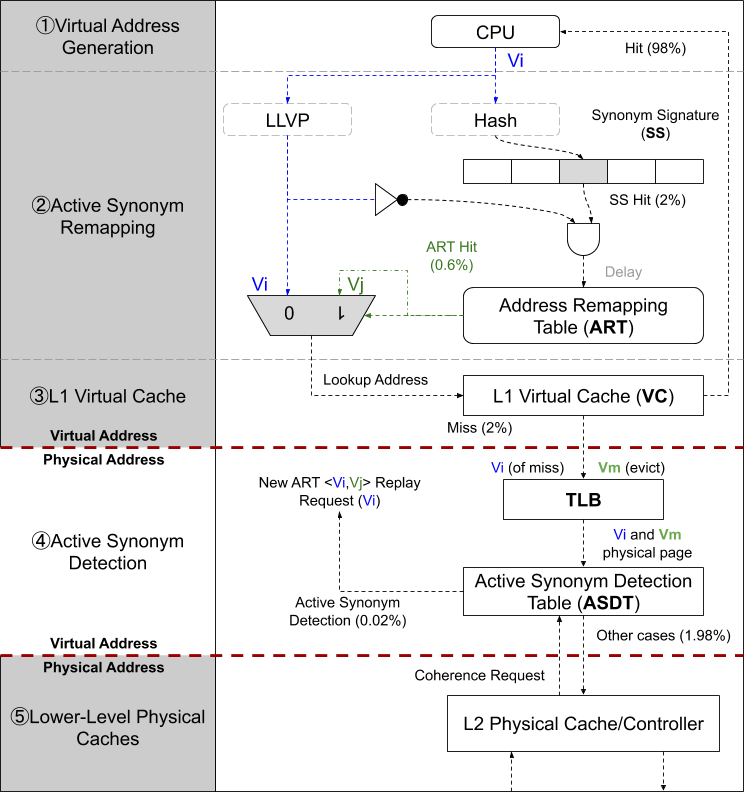
\includegraphics[width=\textwidth]{images/VC-DSR_Cache}
    \caption{\label{fig:VC-DSR}VC-DSR as diagramed by Yoon and Sohi, with LLVP added.}
\end{figure}

On VC miss, the TLB checks the Active Synonym Detection Table (ASDT) to determine if the virtual page is known to correspond to a physical page in cache.  If not, the caching system makes further requests to L2 cache or performs a page table walk.  If the virtual page ultimately does reference a physical page already in cache, the cache arbiter hashes the page, sets the corresponding bit in SS, increments a counter for this bit, and inserts the virtual page into the AST as a synonym to the LVP.

The Last LVP (LLVP) optimization, shown in \prettyref{fig:VC-DSR}, stores the last leading virtual page and requested page in a register, along with metadata.  If the requested address matches the last requested address, the cache arbiter can immediately check metadata (read or write permission) and mux the LVP from this register.  Consecutive memory accesses to the same synonym page skip the AST check; the SS check occurs in parallel, but adds no delay and has no effect.

RISC-V provides a Global bit in the PTE.  The cache arbiter ignores the ASID for Global pages, placing no entry in the SS or AST for the same virtual page in different ASIDs.  Synonyms mapped at alternate virtual addresses are treated as normal.  On IA-32 and AMD64, Yoon and Sohi assume the top half of virtual address space is global.
%\part{The Taiga RISC-V Soft Processor}
\chapter{Taiga}

Eric Matthews and Lesley Shannon created
Taiga\footcite{Matthews2017}\footcite{Matthews2017b} "to facilitate research
into heterogeneous processor systems and high performance architectural
features for soft processors."  Their goals included high instruction-level
paralelization (ILP) at competitive operating frequencies (fMax) and area
usage.

In 2017, Taiga ran on a Xilinx Zynq X7CZ020 FPGA at 111MHz in its minimal
without multiply, divide, TLB, MMU, cache, or atomic operations, and 103MHz at
full configuration.  This version also achieved 254MHz on a Xilinx Virtex
UltraScale+ XCVU9P.  The critical path was the write-back data path in all
except the full configuration, which was limited by access to data TLB tags.

In 2019, they tested Quick-Div on a Xilinx Virtex UltraScale+ VCU118 FPGA board
using an XCVU9P-L2FLGA2014E.  They needed Quick-Div to run at 373MHz to stay
out of the critical path—just shy of 50\% higher fMax than they achieved on the
XCVU9P in 2017.  Clearly, they have improved the processor over time.

Nearly 400MHz performance, even on a modern FPGA, is impressive.  Taiga
achieves clock rates comparable to iDEA, yet implements a full RV32 RISC-V
processor capable of running Linux.


\part{Kerberos}
\chapter{Block Diagrams}

% Kerberos overview
\begin{center}
    \begin{tikzpicture}[scale=0.2]
        \tikzstyle{every node}+=[inner sep=0pt]

        \draw (0,0) -- ++(0,4) -- ++(4,0) -- ++ (0,-4) -- ++(-4,0) -- cycle;

    \end{tikzpicture}
\end{center}
\chapter{Pipeline}

\section{Skid Buffer}
I built the Kerberos skid buffer based on excellent explanations at the ZipCPU blog \footcite{ZipCPU.Pipeline}.  \prettyref{fig:pipeline-skid-buffer-fsm} shows the state machine for the skid buffer.  \prettyref{tab:skid-buffer-handshake-state} shows information about each state; as noted on the ZipCPU blog, \inlinecode{$In.Busy = FullBuffer$}.

\afterpage{

\begin{table}[ht]
    \caption{table}{Handshake States} % title of Table
    \centering % used for centering table
    \begin{tabular}{c c c c} % centered columns (4 columns)
        \hline\hline
        State & FullBuffer & Out.Strobe & DataOut \\ [0.5ex] % inserts table

        \hline
        Passthrough & 0 & In.Strobe & Din \\
        Buffer & 1 & In.Strobe & Din \\
        Flush & 0 & 1 & Buffer \\ [1ex]
        \hline
    \end{tabular}
    \label{tab:skid-buffer-handshake-state}
\end{table}

    % Pipeline FSM
\begin{figure}
    \begin{center}
        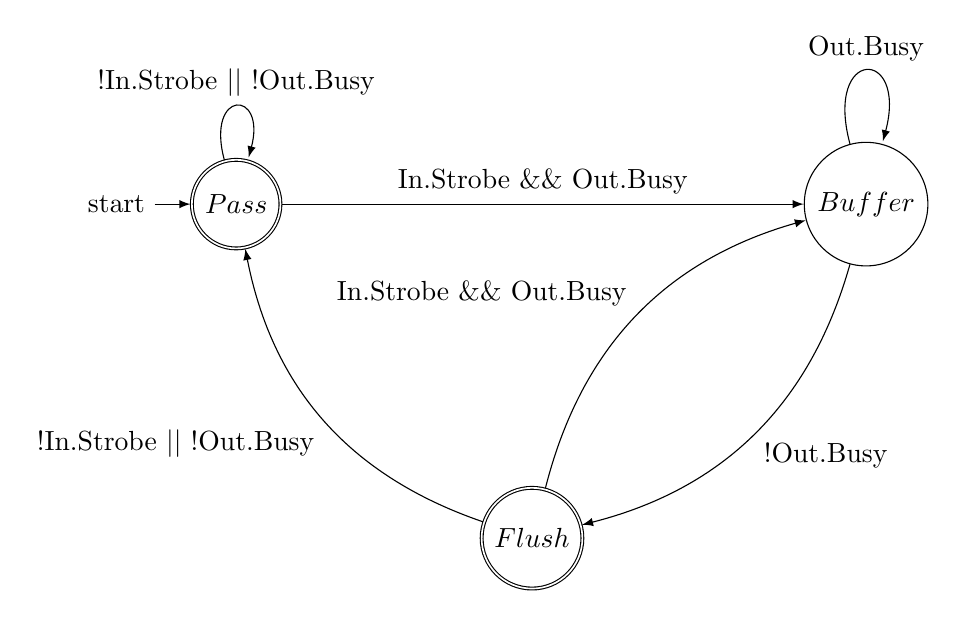
\begin{tikzpicture}[->,>=latex,auto]
    %    \tikzstyle{every node}+=[inner sep=0pt]

        \node[initial,accepting,state] (Pass) {$Pass$};
        \node[state] (Buf) [right of=Pass, node distance=8cm] {$Buffer$};
        \node[accepting,state] (Flush) [below left of=Buf, node distance=6cm] {$Flush$};

        \path (Pass)  edge [loop above] node {!In.Strobe $||$ !Out.Busy} (Pass)
                      edge node {In.Strobe \&\& Out.Busy} (Buf)
              (Buf)   edge [loop above] node {Out.Busy} (Buf)
                      edge [bend left] node {!Out.Busy} (Flush) % Bend right
              (Flush) edge [bend left] node {In.Strobe \&\& Out.Busy} (Buf)
                      edge [bend left] node {!In.Strobe $||$ !Out.Busy} (Pass);
        \end{tikzpicture}
        \caption{Handshake State Machine}
    \end{center}
    \label{fig:pipeline-skid-buffer-fsm}
\end{figure}
}

Pipeline stages signal $Busy$ whenever they are in the $Run$ or $Wait$ states.  A circuit is in the $Run$ state while it is processing, and in the $Wait$ state when it has data sitting on its output but the next stage remains $Busy$.  When the circuit is neither strobing to the next circuit nor processing, it becomes $Idle$, and is not $Busy$ even if the next stage becomes $Busy$. This produces four states:  Idle, Run, Wait, and Finish, shown in \prettyref{tab:pipeline-exec-circuit-state}.

The circuit passes its data on in the Finish state, and is idle on the next iteration; however, the busy signal is \inlinecode{Processing || (DataReady \&\& PipeIn.Busy)}, and so signals \inlinecode{!Busy} on the cycle on which it delivers data.  The \inlinecode{SkidBuffer} itself must accept the data and, besides, is \inlinecode{!Busy} when its buffer is empty and will not magically become busy.

\afterpage{
\begin{table}[ht]
    \caption{Execution Circuit Handshake States} % title of Table
    \centering % used for centering table
    \begin{tabular}{c c c c c} % centered columns (4 columns)
        \hline\hline
        State & Processing & DataReady & PipeOut.Busy & PipeIn.Busy \\ [0.5ex] % inserts table

        \hline
        Idle & 0 & 0 & X & 0 \\
        Run & 1 & 0 & X & 1 \\
        Wait & 0 & 1 & 1 & 1 \\
        Finished & 0 & 1 & 0 & 0 \\ [1ex]
        \hline
    \end{tabular}
    \label{tab:pipeline-exec-circuit-state}
\end{table}
\begin{figure}
    \begin{center}
        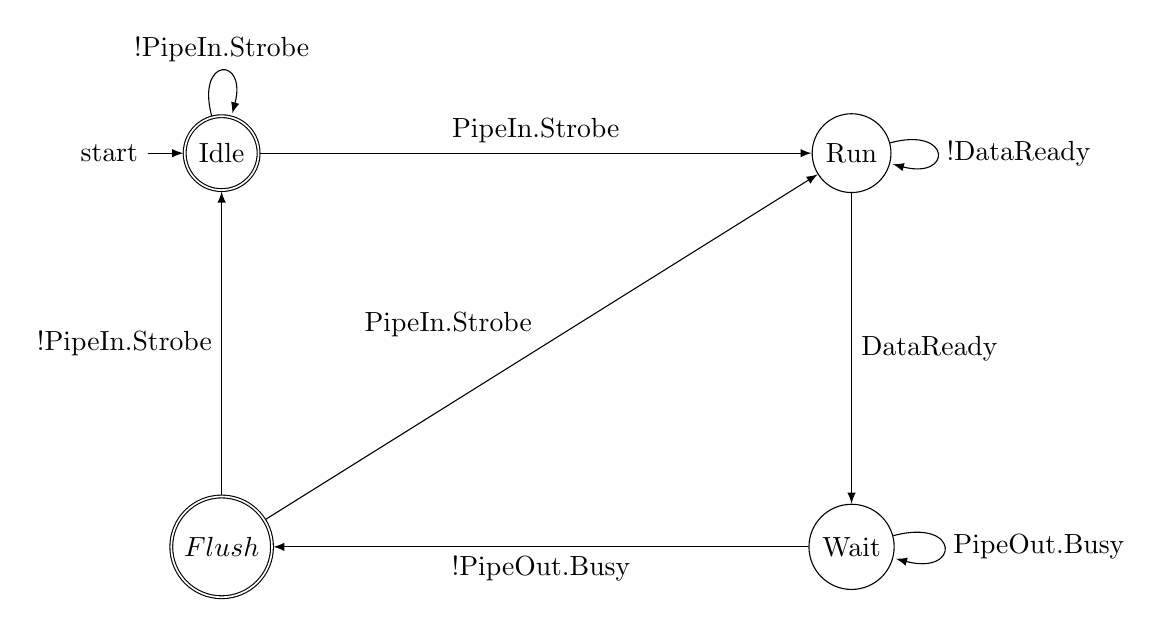
\begin{tikzpicture}[->,>=latex,auto]
            %    \tikzstyle{every node}+=[inner sep=0pt]

            \node[initial,accepting,state] (Idle) {Idle};
            \node[state] (Run) [right of=Idle, node distance=8cm] {Run};
            \node[state] (Wait) [below of=Run, node distance=5cm] {Wait};
            \node[accepting,state] (Finish) [below of=Idle, node distance=5cm] {$Flush$};

            \path (Idle)   edge [loop above] node {!PipeIn.Strobe} (Pass)
            edge node {PipeIn.Strobe} (Run)
            (Run)    edge [loop right] node {!DataReady} (Run)
            edge node {DataReady} (Wait)
            (Wait)   edge [loop right] node {PipeOut.Busy} (Wait)
            edge node {!PipeOut.Busy} (Finish)
            (Finish) edge node {PipeIn.Strobe} (Run)
            edge node {!PipeIn.Strobe} (Idle);
        \end{tikzpicture}
        \captionof{figure}{Execution Circuit Handshake State Machine}
    \end{center}
\end{figure}
}

\section{Fetch}

The \inlinecode{Fetch} stage obtains new instructions and passes them through the pipeline.  It can pass forward large amounts of data—one or several cache lines—containing several instructions, along with the value of \inlinecode{pc} after a branch.  \inlinecode{Fetch} always retrieves and passes along a chunk of instruction stream aligned to its chunk size.

\section{Pre-Decode}

\inlinecode{Pre-Decode} prepares the instruction stream for \inlinecode{Decode}.  It receives instruction stream from \inlinecode{Fetch} one chunk at a time, and tracks \inlinecode{pc} to identify the current address.

\inlinecode{Pre-Decode} converts RISC-V Compressed instructions (RVC) to normal RISC-V instructions.  RVC includes all opcodes with the two least-significant bits not equal to \inlinecode{11}, so \inlinecode{Decode} can ignore these two bits.  This allows cheap handling of \inlinecode{C.JAL} and \inlinecode{C.JALR}:  RVC passes the lower two bits of the opcode forward as-is, and the \inlinecode{Branch} circuit adds 2 rather than 4 to \inlinecode{pc} when these bits are not \inlinecode{11}.

\inlinecode{Pre-Decode} separates each quadrant of RVC into an independent combinational circuit and selects the output via a mux.

Whether expanded from RVC or passed forward verbatim, \inlinecode{Pre-Decode} assembles a single 32-bit instruction with its context information for \inlinecode{Decode}.

\section{Decode}

\inlinecode{Decode} converts instructions to an internal bundle of signals indicating the operation, width, signed or unsigned nature, and instruction layout type.  Like \inlinecode{Pre-Decode}, groups of logically-similar instructions execute as independent combinational circuits and raise a signal to indicate an identified instruction.

Often a single opcode maps to only one or two formats, and the \inlinecode{funct3} and \inlinecode{funct7} fields indicate data width, sign, or modes such as shift-right or subtract, so these circuits are quite compact in gate logic.  A 5-LUT can decode an opcode, and often a 5-LUT or 6-LUT can look up the remaining information—often one bit in the opcode, three from \inlinecode{funct3}, and one from \inlinecode{funct7}.  This minimizes the logic used on FPGAs.

\section{Order}

\section{Load}

\section{Execute}

Small numbers above and below the execute operation indicate the number of cycles and the latency per execution unit.  For example, if the execution stage contains two dividers, the latency can be one cycle rather than however long it takes for the divider to complete.

The \inlinecode{Branch} and \inlinecode{Load/Store} operations use the ALU for simultaneous addition and comparison.  A speculative adder will occasionally run for two cycles, in which case so will \inlinecode{Load/Store}.  Tight loops use backwards branches and suffer a significant performance loss if the addition requires an extra cycle; therefor the ALU supplies two comparators, and the \inlinecode{Branch} unit caches the address of the prior interpreted branch instruction.  \inlinecode{Branch} jumps to the the cached target address if the branch condition and prior branch instruction match, avoiding the adder for all but the first iteration of a tight loop.

\section{Memory Access and Cache}

\inlinecode{Memory Access} also forwards register loads back through the pipeline.  Both \inlinecode{MemoryAccess} and \inlinecode{Fetch} connect directly to VC-DSR L1 cache.
\chapter{Parallelism and Fusing}

Kerberos supplies no single instruction, multiple data (SIMD) instructions, relying on instruction-level parallelization and an instruction fusing approach.
\backmatter
% bibliography, glossary and index go here.
%\printbibliography
\end{document}